\documentclass[oneside,titlepage,a4paper]{Definition/retrospy} %book,article,report,letter


\begin{document}

\title{\Huge\textbf{Research On GameSpy Protocol}} 
\author{Arves100, Xiaojiuwo}


%\date{} %%如果没有这句,会生成时间

\maketitle  %%生成书名

\tableofcontents  %%生成目录

%\mainmatter %%表示文章的正文部分,在生成目录后将从第一页开始

\part{Research On GameSpy SDK}

\chapter{GameSpy General Construction}
\par In GameSpy SDK there are 9 modules, which constructed the GameSpy main functions.
\section{GameSpy SDK Module}
\begin{itemize}
	\item GameSpy Presence Connection Manager
	\item GameSpy Presence Search Player
	\item Nat Negotiation
	\item Query Report 2
	\item Server Browser
	\item Game Patching 
	\item Master Server Patching 
	\item Game Stats and Tracking 
	\item Chat 
\end{itemize}
\subsection{Basic Descriptions of Protocol}
In this part, we show the basic descriptions of protocol in GameSpy Presence SDK.
\subsubsection{The String Pattern}
We first introduce the pattern of the string, which is using to make up a request.
This kind of string is represent a value in a request sends by the client as Table \ref{Value string}.

\begin{table}[H]
	\centering
	\begin{tabular}{|c|c|}
		\hline 
		\textbf{String}&\textbf{Description}  \\ 
		\hline 
		$ \backslash \langle content \rangle \backslash $& The value is $ \langle content \rangle $  \\ 
		\hline 
	\end{tabular} 
	\caption{Value string}
	\label{Value string}
\end{table}

This kind of string is represent a command in a request sends by the client as Table \ref{Command string}. The command will end with $ \backslash \backslash $ or $ \backslash $ depends on whether run at the server-side or client-side.


\begin{table}[H]
	\centering
	\begin{tabular}{|c|c|}
		\hline 
		\textbf{String}&\textbf{Description}  \\ 
		\hline 
		$ \backslash command \backslash\backslash $& This is a command \\ 		
		\hline 
		$ \backslash error \backslash \backslash $ & Error command \\
		\hline
		$\backslash lc \backslash$& Login command\\
		\hline
	\end{tabular} 
	\caption{Command string}
	\label{Command string}
\end{table}



\chapter{The Detail of GameSpy Presence SDK}
\section{GameSpy Presence Connection Manager}
\par GameSpy Presence SDK contain two server, GameSpy Presence Connection Manager (GPCM) and GameSpy Presence Search Player (GPSP). GPCM is a server that handle login request and response with corresponding user information stored on GameSpy. GPSP is a server that handle search request for user.
\subsection{Server IP and Ports}
Table \ref{IP and Ports for GPCM} are the GPCM and GPSP IP and Ports that client/game connect to.
\begin{table}[H]
	\centering
	\begin{tabular}{|c|c|}
		\hline 
		\textbf{IP}&\textbf{Port}\\ 
		\hline 
		gpcm.gamespy.com&29900 \\ 
	 	\hline 
	\end{tabular} 
\caption{IP and Ports for GameSpy Presence Servers}
\label{IP and Ports for GameSpy Presence Servers}

\end{table}
\subsection{Request For GameSpy Presence Connection Manager}
Table \ref{Request For GameSpy Presence Connection Manager} lists the request(already known by us) that clients send to GameSpy Presence Connection Manager server (GPSP).
\begin{table}[H]
	\centering
	\begin{tabular}{|c|c|}
		\hline 
		\textbf{Commands}&\textbf{Description}  \\ 
		\hline 
		$\backslash inviteto \backslash\backslash$& Invite friends\\ 		
		\hline 
		$\backslash login \backslash\backslash$&Login to GPCM \\
		\hline
 		$\backslash getprofile \backslash\backslash$&	Get profile of some player\\
 		\hline
		$\backslash addbuddy \backslash\backslash$& Add player to my friend list \\
		\hline
		$\backslash delbuddy \backslash\backslash$ & Delete player from my friend list \\
		\hline
		$\backslash updateui \backslash\backslash$& ?\\
		\hline
		$\backslash updatepro \backslash\backslash$& Update player's profile such as first name, last name, gender etc. \\
		\hline
		$\backslash logout \backslash\backslash$& Logout manually by user\\
		\hline
		$\backslash status \backslash\backslash$& Update status of a user\\
		\hline
		$\backslash ka \backslash\backslash$& Keep client alive(do not disconnect) \\
 		
		\hline 
	\end{tabular} 
	\caption{Request For GameSpy Presence Connection Manager}
	\label{Request For GameSpy Presence Connection Manager}
\end{table}

Error response string for (GPCM, GPSP):
\begin{equation}
\begin{split}
\backslash error \backslash\backslash err \backslash \langle error code \rangle \backslash fatal\backslash\backslash errmsg \backslash \langle error message \rangle \backslash id\backslash 1 \backslash final \backslash
\end{split}	
\end{equation}
\subsubsection{Login Phase}
\myparagraph{Client Login Request}
There are three ways of login:
\begin{itemize}
	\item AuthToken: Logging using an alphanumeric string that rapresents an user
	\item 	UniqueNick: Logging using a nickname that is unique from all the players
	\item User: Logging with the nickname and the password
\end{itemize}

The full login request string:
\begin{equation}\label{Chanllenge string}
\begin{split}
	&\backslash login \backslash challenge \backslash \langle challenge \rangle \backslash authtoken \backslash \langle authtoken \rangle \\& \backslash uniquenick \backslash \langle uniquenick \rangle \backslash user \backslash \langle user \rangle 
	\backslash userid \backslash \langle userid \rangle \\& \backslash profileid \backslash \langle profileid \rangle \backslash partnerid \backslash \langle partnerid \rangle \backslash response \backslash \langle response \rangle \\&
	 \backslash firewall \backslash 1 \backslash port \backslash \langle port \rangle \backslash productid \backslash  \langle productid \rangle \\& \backslash gamename \backslash \langle gamename \rangle \backslash namespaceid \backslash \langle namespaceid \rangle \\& \backslash  sdkrevision \backslash \langle sdkrevision \rangle \backslash quiet \backslash \langle quiet \rangle \backslash id \backslash 1 \backslash final \backslash
\end{split}
\end{equation}
The value $ \langle challenge \rangle $ for $ \backslash challenge \backslash $ in \ref{Chanllenge string} is a 10 byte alphanumeric string.

The following Table \ref{Login parameter string} is a description of string used in login request, GameSpy can use these string to find value in database.
\begin{table}[H]
	\centering
%\begin{tabular}{A}

\begin{tabular}{A}
		\hline
		\textbf{Keys} & \textbf{Description} & \textbf{Type}
			                                                                          \\ \hline
		 login& The login command which use to identify the login request of client&\\ \hline
		 challenge  & The user challenge used to verify the authenticity of the client     &                                                                                                                                     \\ \hline
		 authtoken  & The token used to login (represent of an user)        &                                                                                                                                                    \\ \hline
		uniquenick  & The unique nickname used to login       &                                                                                                                                                                  \\ \hline
		   user     & The users account (format is NICKNAME@EMAIL)           &                                                                                                                                                   \\ \hline
		  userid    & Send the userid (for example when you disconnect you will keep this)              &                                                                                                                        \\ \hline
		 profileid  & Send the profileid (for example when you disconnect you will keep this)           &                                                                                                                        \\ \hline
		 partnerid  & This ID is used to identify a backend service logged with gamespy.(Nintendo WIFI Connection will identify his partner as 11, which means that for gamespy, you are logging from a third party connection) &\\ \hline
		 response   & The client challenge used to verify the authenticity of the client     &                                                                                                                                   \\ \hline
		 firewall   & If this option is set to 1, then you are connecting under a firewall/limited connection &\\
		 \hline
		 port& The peer port (used for p2p stuff)            &                                                              \\ \hline
		 productid  & An ID that identify the game you're using            &                                                                                                                                                     \\ \hline
		 gamename   & A string that rapresents the game that you're using, used also for several activities like peerchat server identification             &                                                                    \\ \hline
		
		namespaceid & ?   &                                                                                                                                                                                                      \\ \hline
		sdkrevision & The version of the SDK you're using& \\ \hline
		   quiet    & ? Maybe indicate invisible login which can not been seen at friends list &\\ \hline
		   id& The value is 1&\\ \hline
		   final & Message end&\\ \hline
	\end{tabular} 
	\caption{Login parameter string}
	\label{Login parameter string}
\end{table}
\paragraph{Login Response From Server}\mbox{}\\

This response string \ref{Login response string1}, \ref{Login response string2} is send by the server when a connection is accepted, and followed by a challenge\ref{Chanllenge string}, which verifies the server that client connect to.
\par There are two kinds of login response string: 
\begin{equation}\label{Login response string1}
\begin{split}
&\backslash lc \backslash 1 \backslash challenge \backslash \langle challenge \rangle \backslash nur \\&\backslash userid \backslash \langle userid \rangle \backslash profileid \backslash \langle profileid \rangle \backslash final \backslash
\end{split}	
\end{equation}

\begin{table}[H]
	\centering
	\begin{tabular}{A}

		\hline 
		\textbf{Keys}&\textbf{Description}&\textbf{Type}  \\ 
		\hline 
		challenge & The challenge string sended by GameSpy Presence server&  \\ 		
		\hline 
		nur & ? &\\
		\hline 
 userid&The userID of the profile &\\	\hline 
 profileid&The profileID &\\	\hline 
 final& &\\	\hline 
	\end{tabular} 
	\caption{The first type login response}
	\label{The first type login response}	
\end{table}

\begin{equation}\label{Login response string2}
\begin{split}
&\backslash lc \backslash 2 \backslash sesskey \backslash \langle sesskey \rangle  \backslash userid \backslash \langle userid \rangle \backslash profileid \backslash \langle profileid \rangle \\& \backslash uniquenick \backslash \langle uniquenick \rangle \backslash lt \backslash \langle lt \rangle \backslash proof \backslash \langle proof \rangle \backslash final \backslash
\end{split}	
\end{equation}

\begin{table}[H]
	\centering
	\begin{tabular}{A}
		\hline 
		\textbf{Keys}& \textbf{Description}&\textbf{Type}  \\ 
		\hline 
		sesskey & The session key, which is a integer rapresentating the client connection& \\ 		
		\hline 
		userid & The userID of the profile& \\
		\hline 
		profileid&The profileID &\\	\hline 
		uniquenick&The logged in unique nick &\\	\hline 
		lt& The login ticket, unknown usage&\\\hline
		proof& The proof is something similar to the response but it vary&\\\hline
		final& &\\
	\hline 
	\end{tabular} 
	\caption{The second type login response}
	\label{The second type login response}
\end{table}
Proof in \ref*{The second type login response} generation: $ md5(password)||48 spaces $
The user could be AuthToken or the User/UniqueNick (with the extra PartnerID).
server challenge that we received before.
the client challenge that was generated before.




\subsubsection{User Creation}
This commmand \ref{Create user command} is used to create a user in GameSpy.
\begin{equation}\label{Create user command}
\begin{split}
&\backslash newuser \backslash email \backslash \langle email \rangle \backslash nick \backslash \langle nick \rangle \\& \backslash passwordenc \backslash \langle passwordenc \rangle 
\backslash productid \backslash \langle productid \rangle \\& \backslash gamename \backslash \langle gamename \rangle \backslash uniquenick \backslash \langle uniquenick \rangle \\& \backslash cdkeyenc \backslash \langle cdkeyenc \rangle \backslash partnerid \backslash \langle partnerid \rangle \backslash id \backslash 1 \backslash final \backslash
\end{split}	
\end{equation}
The description of each parameter string is shown in Table \ref{User creation string}.
\begin{table}[H]
	\centering
	\begin{tabular}{A}
		\hline
		  \textbf{String}    & \textbf{Description} &\textbf{Type}                                                                 \\ \hline
		   email    & The email used to create                                                    & \\ \hline
		   nick     & The nickname that will be created                                            & \\ \hline
		passwordenc & The encoded password (password XOR with Gamespy seed and the Base64 encoded)  &\\ \hline
		 productid  & An ID that identify the game you're using                                     &\\ \hline
		 gamename   & A string that rapresents the game that you're using, used also for several    &\\ \hline
		namespaceid & ?Unknown                                                                      &\\ \hline
		uniquenick  & Uniquenick that will be created                                               &\\ \hline
		 cdkeyenc   & The encrypted CDkey, encrypted method is the same as the passwordenc          &\\ \hline
		 partnerid  & This ID is used to identify a backend service logged with gamespy             &\\ \hline
		    id      & The value of id is 1                                                          &\\ \hline
		   final    & Message end                                                                   &\\ \hline
	\end{tabular}
\caption{User creation string}
\label{User creation string}
\end{table}

\section{GameSpy Presence Search Player}
Table \ref{IP and Port for GPSP} are the GPSP IP and Ports that client/game connect to.
\begin{table}[H]
	\centering
	\begin{tabular}{|c|c|}
		\hline 
		\textbf{IP}&\textbf{Port}  \\ 		
		\hline 
		gpsp.gamespy.com&29901 \\
		\hline 
	\end{tabular} 
	\caption{IP and Ports for GameSpy Presence Search Player}
	\label{IP and Ports for GameSpy Presence Search Player}
	\end{table}
\subsection{Search User}
This is the request that client sends to server:
\begin{equation}\label{Search User Request}
\begin{split}
 \backslash search\backslash\backslash sesskey \backslash<sesskey>\backslash profileid \backslash <profileid> \\ \backslash namespaceid\backslash <namespaceid>  \backslash partnerid\backslash <partnerid>\\ \backslash nick \backslash <nick> \backslash uniquenick \backslash <uniquenick> \\ \backslash email \backslash <email> \backslash gamename \backslash <gamename> \backslash final \backslash
\end{split}
\end{equation}

This is the response that server sends to client:
\begin{equation}
	\begin{split}
	\backslash bsr \backslash <profileid> \backslash nick \backslash <nick>	\backslash uniquenick \backslash <uniquenick> \\
	\backslash namespaceid \backslash <namespaceid>\backslash firstname \backslash <firstname> \\ 
	\backslash lastname \backslash <lastname>\backslash email \backslash <email> \\
	\backslash bsrdone \backslash <gamespy enc determinator> \backslash final \backslash
	\end{split}
\end{equation}
\section{GameSpy Status and Tracking}
when game connect to GSTATS server, server will send an message to game which contains the challenge, the total length of message must bigger than 38bytes, and the challenge must bigger than 20bytes.
when game received the challenge it will compute a response, the response is formed as follows. 
response = CRC32(<server challenge>,<length of server challenge>)||<game secret key>
then game will compute the MD5 hash as MD5value = MD5(<response>,<length of response>)
then encoded with Enctype3
then construct the challenge-response message as $ \backslash auth \backslash \backslash gamename \backslash <gamename>\backslash response \backslash <MD5value> \backslash port \backslash <port> \backslash id \backslash <id> $

session key length (unknown)
connction id = transfer ascii of sessionkey to integer

the initialization phase is finished.
server challenge message length (bigger than 38-byte)
server challenge length (bigger than 20-byte)
$ \backslash final \backslash $ is encrypted using XOR Enctype1 at the end of the challenge that sends by the server.

\part{RetroSpy System Architecture}



\chapter{Introduction}
2014 is a year that thousands games are abandon by GameSpy. I still remember the day when GameSpy shutdown, no matter how hard i try to login into Crysis2 multiplayer, but the same error shows "An error has occurred. Please check your network connectivity"\ref{Crysis2 error message}.
\begin{figure}[H]
	\centering
	\caption{Crysis2 error message}
	\label{Crysis2 error message}
	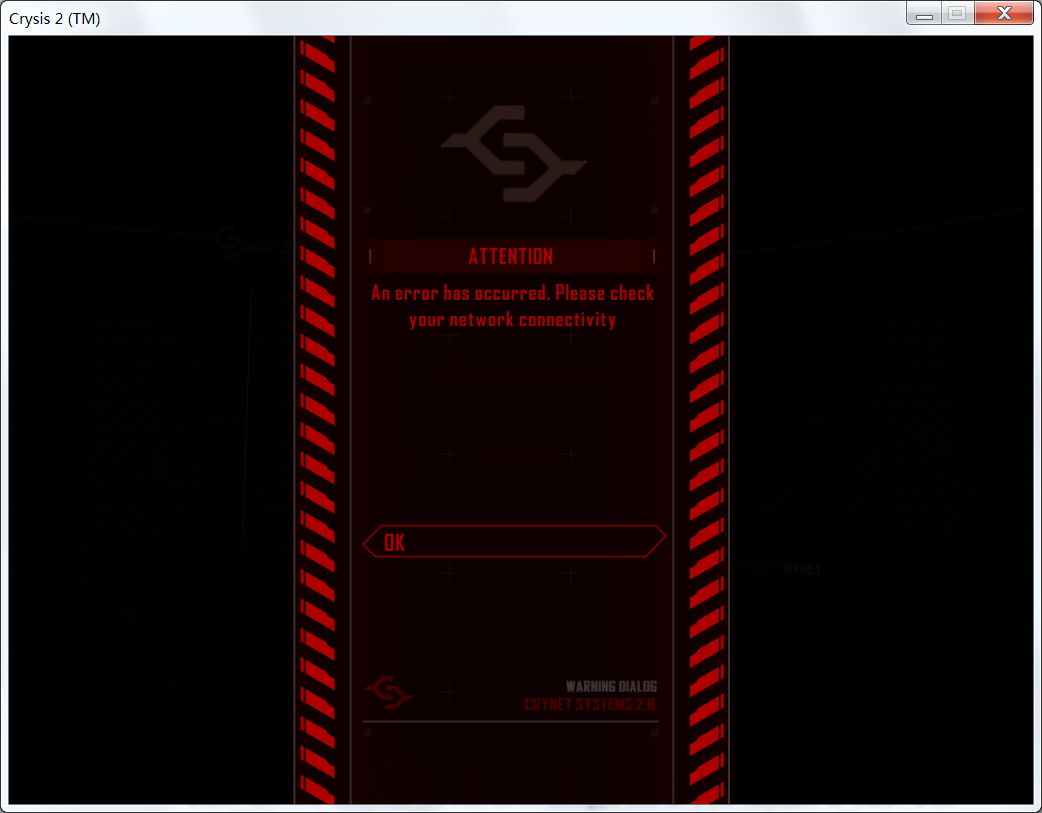
\includegraphics[scale=0.25]{Pictures/Crysis2error.png}
\end{figure}

\chapter{Database}
This kind of string is represent a parameter in a request sends by the client \ref{Parameter string}. GameSpy uses the combination of the parameter to search the string with value, and sends the data back to client use this kind of parameter string.
\subsection{Database Key Field}
These keys is that GameSpy Presence SDK using to find a user in their database. Keys are shown in Table \ref{Key Field}.

\begin{table}[H]
	\centering
	\begin{tabular}{|c|>{\centering\arraybackslash}p{8cm}|}
		\hline 
		\textbf{Keys}& \textbf{Description}  \\ 
		\hline 
		$user$ & An user contains the Email and the password, but contains multiple profiles \\ 		
		\hline 
		$profileid$ & The profile contains the name, surname, birth date and all the rest user info, including
		an unique nickname used to identify the profile and a generic nickname used to show for example in
		games \\
		\hline 
	\end{tabular} 
	\caption{Key Field}
	\label{Key Field}	
\end{table}

\begin{table}[H]
	\centering
	\begin{tabular}{|c|c|}
		\hline 
		\textbf{String}&\textbf{Description}  \\ 
		\hline 
		$ \backslash id \backslash 1 \backslash $& This is a parameter string the value of $ id $ is $ 1 $ \\ 		
		\hline 
		$ \backslash profileid \backslash 007 \backslash $ & This is a parameter string the value of $ profileid $ is $ 007 $ \\
		\hline
	\end{tabular} 
	\caption{Parameter string}
	\label{Parameter string}
\end{table}

\chapter{The Detail of RetroSpy Project}
All projects in the RetroSpy visual studio solution is listed as follows.
\begin{itemize}
	\item GameSpyLib: The library for all RetroSpy servers.
	\item CDKey: CD-Key server.
	\item NATNegotiation: NAT negotiation server.
	\item PresenceConnectionManager: GPCM server.
	\item PresenceSearchPlayer:  GPSP server.
	\item QueryReport: Query report server.
	\item ServerBrowser: Server browser server.
	\item StatsAndTracking: Stats and tracking server.
	\item SAKEPersistentStorage: SAKE persistent storage server.
\end{itemize}
\section{GameSpyLib}
	\subsection{Common}
	\subsection{Database}
	\subsection{Extensions}
	\subsection{Logging}
	\subsection{Networks}
	There are two different servers in RetroSpy; one is TCP another is UDP.  TCP and UDP work differently so the implementation will be different. We show the different implementing in \ref{Tcp} and \ref{Udp}.
	\subsubsection{Tcp}\label{Tcp}
	TcpServer class is only for making the connection and listening for connections. TcpStream is for receiving and sending the message.
	\subsubsection{Udp}\label{Udp}
	UdpServer class does not need a server to handle connection and listen for connection, every client can be a server, and every server is a client. So this class has both receiving and sending functions.

\section{CDKey}
\section{NATNegotiation}
\section{PresenceConnectionManager}
\subsection{LoginHandler}
Different game will have different request. Some of request contain different combination of <key,value> pairs. The request we already known is shown in the Table~\ref{Game requests key}.
\begin{table}[H]
	\centering
	\begin{tabular}{|c|c|}
		\hline 
		\textbf{Game name}&\textbf{request}  \\ 
		\hline 		
		armada2 & firewall,port \\
		\hline
		gslive& uniquenick,productid,partnerid,gamename,sdkrevision \\ 		
		\hline 
		Crysis2&uniquenick,productid,partnerid,gamename,sdkrevision \\
		\hline
	\end{tabular} 
	\caption{Game requests key}
	\label{Game requests key}
\end{table}
\section{PresenceSearchPlayer}
\subsection{NewUserHandler}

\section{QueryReport}
\section{ServerBrowser}
\section{StatsAndTracking}
\section{SAKEPersistentStorage}

\chapter{conclusion}

\end{document}
